\iffalse
\section{Rethinking the Internet experience}
%I HAVE A DREAM
Cloud computing
\\Modularity
\\anonymity, privacy
\\authentication, accountability, encryption, security
\\no middlewares
\\TCP/IP stack data, controller functionality
\\subnetworks
\\mobility and multihoming
\\independent from organizations
\fi



\newpage
\section{Software Defined,\\ Service-centric Networking}
A well thought Service centric architecture provides two things:
\begin{enumerate} \itemsep1pt \parskip0pt 
\parsep0pt
  \item the right abstractions for services, for developers and users to use
  \item a service-aware data/control plane split
\end{enumerate}

\begin{figure}[H]
\centering
\phantomsection
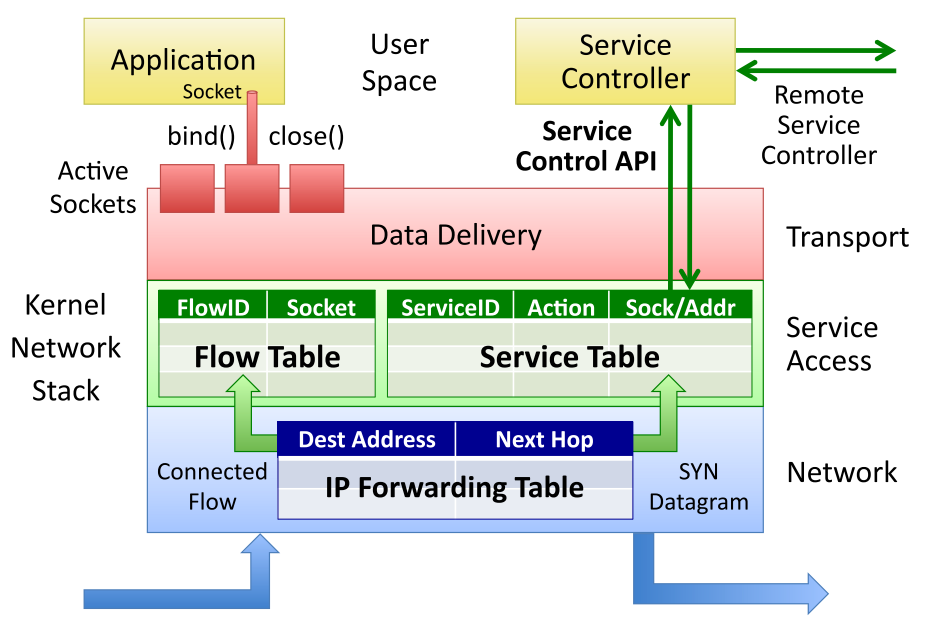
\includegraphics[scale=0.3]{figures/SAL_plane_split}
\caption[Control/Data plane separation in Serval]{Control/Data plane separation in Serval. Data plane service routing roules are stored in the Service table residing in SAL, while control plane logic is implemented in the Service Controller.}
\label{fig:sal_plane_split}
\end{figure}

Confidently, Serval provably does well with both.
This makes us sceptical on if the control plane could be in a way merged with software defined networking APIs.
That way, the network stack could have control over the fabric of the network.
And service-related events could be propagated to SDN-enabled devices as well.

This is the concept behind Service-Aware Networking; 
Software Defined Networking could benefit from Serval's data/control plane separation and enable services running in – possibly distributed – datacenters to automatically, and according to the rights they have been granted, manipulate networks to better utilize the underlying network infrastructure, conforming to their dynamic needs.
In other words, applications using active sockets will be able to modify network topology, co-working with the Service Controller and a centralized SDN controller.
This way, Serval can enable SDN reach the end-host nodes, very much alike SDN-ready applications are currently doing.

A great potential is hidden behind the way service-level routing rules management can be propagated with the use of Service Controllers.
Specifically immediate, network-wide changes are possible with any modification in the Service table or with lower links going up and down.

Actually Serval has in a way its own counterpart software defined API, the \emph{Service Control API}.
One can say so, taking a look in the way Service Controllers are exchanging information with each other and with the Serval Routers.
The integration though with a well-established API, such as Openflow \cite{McKeown2008}, will provide the flexibility of managing OpenFlow switches devices, and writing routing rules on host/interface and service instance changes, in a dynamic policy-driven manner.

\subsection{Scenario: Service Registration as a Network Policy}
Let us imagine a simple case scenario in a datacenter network, which could benefit from the integration of OpenFlow APIs in a Serval-compatible controller.

A POX\footnote{POX is a platform for the rapid development and prototyping of network control software using Python, providing OpenFlow interfaces.\\ \url{http://www.noxrepo.org/pox/about-pox/}} controller is listening for Service Registrations.
Once the instance of a service binds on an active socket with a serviceID, let's say, serviceX, a service registration event is triggered in SAL, a DEMUX rule is added in SAL's service table and the Service Controller is activated.

The Service Controller of that machine is using Serval's Service Control API to notify other Serval-enabled nodes for the new instance.
The Service Controllers of the other machines who receive that message, add a rule for forwarding SYN packets with the destination serviceID equal to serviceX, to the machine which originated the service registration.
If there are other instances of the same service, then the IP address of the machine is added to the relative list of IPs for forwarding.

The Service Controller of the server running the service instance is also informing the SDN controller which is controlling the OpenFlow switches network fabric.
Since the SDN controller has a rule for making serviceX instances available to the outer world, forwarding rules are added in OpenFlow switches for creating paths for packets coming from away the datacenter.

Immediately and without human intervention, as soon as an interface binds on an active socket, it can start listening on requests from clients.
And this functionality is achieved by service-aware networking, mainly with the control-plane mechanisms provided by the service-centric architecture.

A similar case with a virtual machine\nomenclature{VM}{Virtual Machine} migration can be thought.
Serval's in-band signalling can maintain the connection of an active-socket and notify the other end about the new IP address.
Service Controller can inform the SDN controller to create the datapath from external clients to reach the VM with the new IP.
In no time, the VM service instance is ready to serve both existing and new clients, without resetting original sockets state.



\iffalse
\newpage
\section{Service-Aware Networking and Cloud Networks}
How can we take advantage of the above mentioned results in cloud networks?
why cloud fits the description
\fi

\iffalse
\newpage
\section{Introduction to the Proposed Solution}
User Serval as it is, but with a Distributed Service Resolution Service
\\Based on DHT algorithms
\\Run by tier-1 and ISPs, or by users in Autonomous networks
\\Secure identifiers
\\Flat namespace
\\Gets serviceID and
\\- either returns the (IP,Port) back to the client
\\- or forwards the packet directly to the service provider
\\- caches the (serviceID, IP) tuple for future use
\\Incrementally deployable and backwards compatible
\\written in C, running in the user space
\\accept service registration, checks HIP and inform the relative nodes
\\About the Service Controller:
\\will be running as a daemon in the userspace
\\will communicate with ServalDHT to resolve serviceIDs (hashed service names)
\\will enable delegation, load balancing etc as modules (maybe a configuration file?)
\\Draw a FSM for the SRS \nomenclature{SRS}{Service Resolution Service} (http://madebyevan.com/fsm/)
\fi

\newpage
\section{Future Research}
Service-Aware networking is a multi-faceted field, with a lot of research to be done.
We could propose though the continuation of the ideas presented in this thesis with one of the following topics:
\begin{enumerate}
  \item Implement Service Controller (compatible with OpenFlow)
  \item Deployment in PlanetLab or guifinet
  \item Serval router as a virtualized networking service on cisco nexus
  \item Arrakis ("The Operating System is the Control Plane") and Service-Aware networking
  \item ServalDHT
\end{enumerate}

\subsection{ServalDHT: Secure-DHT based Service Resolution Service for the Serval architecture}
\subsubsection{The challenges of private, hierarchical DNS}
Over time, the Internet has gathered a great power over diverse societies.
People all around the world are trusting in order to read about the news, form a political opinion, solve problems in their working environment, do market research.
However, while the Internet continuously affirms its prominent value, it is a surprise how vulnerable it remains to arbitrary (inter)national control and malicious attacks, due to the fact that it is erringly administered by private organizations and its restrained, hierarchical structure. \\
\indent One of the fundamental components of the the functionality of the Internet is the Domain Name System (DNS).
It is used to map human readable names of hosts to numerical IP addresses needed for the purpose of locating service providers around the world and effectively routing traffic to them.
Those identifiers, called domain names, are annually purchased and assigned through the Internet Registry by the private organization ICANN (Internet Corporation for Assigned Names and Numbers).
In addition to being peremptory, this domination also grants to ICANN the privilege of overseeing the content of Internet, by cutting out or declining registration to "undesirable" domains.
Nevertheless, various incidents of catachresis are being observed the last years, with governments like the Egyptian one that shut down its DNS servers to muzzle the protesters in 2011, and the Chinese which still blacklists certain domains as a mechanism for Internet censorship.\\
\indent Moreover, the current Domain Name Service is based on an hierarchical architecture, where (domain name, IP) tuples are cached in midway servers.
This is causing great problems when a service provider has to renew its IP address, because even if a DNS root server is updated, users still get the old cached IP address yet after hours.
This time delay can increase to days in cases where recursive DNS servers do not follow the specified TTL values for their cached entries.
Consequently, hosts are restrained from taking advantage of functionality like multihoming and (virtual machine) migration.
For the same reason, in cases of machine failure, the failover will take a long time, returning in the meanwhile a server unreachable response. \\
\indent Besides, inevitably imitating the hierarchical architecture for domain resolution, autonomous networks must have exclusive, trusted machines offering an analogous service all the time.
This is not always desired, for example in Metropolitan Area Networks (MAN) \nomenclature{MAN}{Metropolitan Area Networks} where ranking does not make sense.\\
\indent Other problems related to DNS bear upon the lack of a widely adopted protocol to correctly verify the real identity of service hosts.
DNS has been proved fallible to various attacks, like (Distributed) Denial of Service attacks (known as DDoS \nomenclature{DDoS}{Distributed Denial of Service} and DoS \nomenclature{DoS}{Denial of Service} attacks), Cache Poisoning (or DNS Spoofing) etc., which aim on deliberately redirecting requests to malevolent hosts.
